\documentclass{article}
\usepackage{tikz}
\begin{document}
% 画直线、圆、椭圆、长方形、圆弧
\begin{tikzpicture}
    % 直线,两个点
    \draw (0,0) -- (2,0);

    % 圆,圆心和半径
    \draw (0,-2) circle [radius=1];

    % 椭圆,圆心和x/y半径
    \draw (0,-4) ellipse [x radius=1, y radius=.8];

    % 长方形,两个对角线上的顶点
    \draw (0,-10) rectangle (2,-8);

    % 圆弧,起始点、起始/结束角度和半径
    \draw[->] (-1.5,-15) -- (1.5,-15);
    \draw[->] (0,-16.5) -- (0,-13.5);
    \draw (0,-15) circle [radius=1];
    \draw (.5,-15) arc [start angle=0, end angle=120, radius=.5];
    
    % 椭圆弧,起始点、起始/结束角度和x/y半径
    \draw[->] (-2,-20) -- (2,-20);
    \draw[->] (0,-21.5) -- (0,-18.5);
    \draw (0,-20) ellipse [x radius=1.6, y radius=.8];
    \draw (.8,-20) arc [start angle=0, end angle=90, x radius=.8, y radius=.4];
\end{tikzpicture}\vspace{1cm}

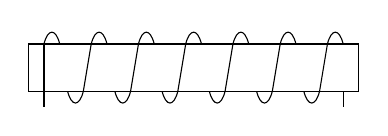
\begin{tikzpicture}
    % 曲线,使用(<first_point>) .. controls (<first_control_point>) and (<second_control_point>) .. (<second_point>)
    % 原理: 第一个点first_point的切线指向第一个控制点first_control_point,第二个点second_point的切线指向第二个控制点second_control_point
    % 如果省略 and (<second_control_point>),则第二个点second_point的切线也指向第一个控制点first_control_point
    \draw (-2,-0.3) rectangle (2.2,0.3);
    \draw (-1.8,-0.5) -- (-1.8,0.3);
    % 螺线
    \foreach \x in {-1.8,-1.2,-0.6,0,0.6,1.2}{
        \draw (\x,0.3) .. controls (\x+0.05,0.5) and (\x+0.15,0.5) .. (\x+0.2,0.3);
        \draw (\x+0.3,-0.3) ..controls (\x+0.35,-0.5) and (\x+0.45,-0.5) .. (\x+0.5,-0.3);
        \draw (\x+0.5,-0.3) -- (\x+0.6,0.3);
    }
    \draw (1.8,0.3) .. controls (1.85,0.5) and (1.95,0.5) .. (2,0.3);
    \draw (2,-0.3) -- (2,-0.5);
\end{tikzpicture}
\end{document}
